%!TEX program = pdflatex
\documentclass[a4paper, 11pt]{article}

% ==================== PACKAGES ====================
\usepackage[utf8]{inputenc}
\usepackage[T1]{fontenc}
\usepackage[english]{babel}
\usepackage{amsmath, amssymb, amsfonts}
\usepackage{graphicx}
\usepackage{float}
\usepackage{booktabs}
\usepackage{array}
\usepackage{tabularx}
\usepackage{multirow}
\usepackage{geometry}
\usepackage{hyperref}
\usepackage{xcolor}
\usepackage{enumitem}
\usepackage{siunitx}
\usepackage{caption}
\usepackage{subcaption}
\usepackage{fancyhdr}
\usepackage{tcolorbox}
\usepackage{physics}

% ==================== GEOMETRY ====================
\geometry{
    left=2.5cm,
    right=2.5cm,
    top=2.5cm,
    bottom=2.5cm,
    headheight=14pt
}

% ==================== COLORS ====================
\definecolor{darkblue}{RGB}{0, 51, 102}
\definecolor{lightblue}{RGB}{230, 240, 250}
\definecolor{darkgreen}{RGB}{0, 100, 0}
\definecolor{darkred}{RGB}{139, 0, 0}
\definecolor{lightyellow}{RGB}{255, 255, 224}

% ==================== HYPERREF SETUP ====================
\hypersetup{
    colorlinks=true,
    linkcolor=darkblue,
    urlcolor=darkblue,
    citecolor=darkblue
}

% ==================== HEADER/FOOTER ====================
\pagestyle{fancy}
\fancyhf{}
\fancyhead[L]{\textit{Fiber Optics - Nonlinearity}}
\fancyhead[R]{\textit{FO10 Summary}}
\fancyfoot[C]{\thepage}
\renewcommand{\headrulewidth}{0.4pt}

% ==================== CUSTOM BOXES ====================
\newtcolorbox{keypoint}{
    colback=lightblue,
    colframe=darkblue,
    fonttitle=\bfseries,
    title=Key Point
}

\newtcolorbox{formula}{
    colback=yellow!10,
    colframe=orange!80!black,
    fonttitle=\bfseries,
    title=Formula
}

\newtcolorbox{physical}{
    colback=green!5,
    colframe=darkgreen,
    fonttitle=\bfseries,
    title=Physical Interpretation
}

\newtcolorbox{warning}{
    colback=red!5,
    colframe=darkred,
    fonttitle=\bfseries,
    title=Important Note
}

% ==================== DOCUMENT ====================
\begin{document}

% ==================== TITLE PAGE ====================
\begin{titlepage}
    \centering
    \vspace*{2cm}
    
    {\Huge\bfseries Nonlinearity in Optical Fibers\\[0.5cm]}
    {\Large\textit{From Maxwell's Equations to Solitons and Modulation Instability}\par}
    
    \vspace{2cm}
    
    {\large Summary of Lecture Notes by Luca Palmieri\par}
    {\large Course: Fiber Optics\par}
    {\large Academic Year 2019/2020\par}
    
    \vspace{3cm}
    
    \begin{abstract}
    This document provides a comprehensive analysis of nonlinear effects in optical fibers, starting from the transition from linear to nonlinear Maxwell equations through the mechanical oscillator model. The document derives the Nonlinear Schrödinger Equation (NLSE) from Helmholtz equation using the slowly varying envelope approximation, and explores in detail the main nonlinear phenomena: Self-Phase Modulation (SPM), Cross-Phase Modulation (XPM), Solitons, and Modulation Instability (MI). Each mathematical formula is accompanied by its physical interpretation and real-world significance.
    \end{abstract}
    
    \vfill
    
    {\large ICT Engineering - Summary Document\par}
    {\large January 2026\par}
\end{titlepage}

\tableofcontents
\newpage

% ==================== INTRODUCTION ====================
\section{Introduction to Nonlinearity}

\subsection{The Linear Regime and Its Limitations}

In the linear regime, the propagation of electromagnetic waves in optical fibers is governed by Maxwell's equations with a linear relationship between the electric field $\vec{E}$ and the polarization $\vec{P}$ of the medium:

\begin{equation}
    \vec{P} = \varepsilon_0 \chi^{(1)} \vec{E}
    \label{eq:linear_polarization}
\end{equation}

\begin{physical}
\textbf{Physical Meaning:} In the linear regime, the polarization (the alignment of electric dipoles in the material) is directly proportional to the applied electric field. This means that doubling the field strength exactly doubles the polarization response. This approximation works well for low optical powers.
\end{physical}

However, when the optical power increases, this linear relationship breaks down. The material's response becomes nonlinear, leading to new phenomena that cannot be explained by linear optics.

\subsection{Why Nonlinearity Matters}

Nonlinear effects in optical fibers are crucial for several reasons:

\begin{itemize}[leftmargin=*]
    \item \textbf{System limitations:} Nonlinearity can degrade signal quality in high-power transmission systems
    \item \textbf{New applications:} Nonlinear effects enable technologies like optical amplification, wavelength conversion, and supercontinuum generation
    \item \textbf{Soliton transmission:} Nonlinearity can be exploited to compensate chromatic dispersion, enabling ultra-long distance transmission
    \item \textbf{Signal processing:} All-optical signal processing relies on nonlinear effects
\end{itemize}

% ==================== MECHANICAL OSCILLATOR MODEL ====================
\section{From Linear to Nonlinear: The Mechanical Oscillator Model}

\subsection{The Classical Harmonic Oscillator}

To understand how nonlinearity arises in optical materials, we use the analogy of a mechanical oscillator. Consider an electron bound to an atom, subjected to an external electric field $E(t)$.

\begin{figure}[H]
    \centering
    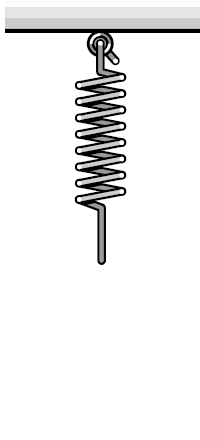
\includegraphics[width=0.5\textwidth]{image-000.png}
    \caption{Mechanical oscillator model showing an electron bound to an atom by a restoring force. The electron displacement $x$ is driven by the external electric field $E(t)$.}
    \label{fig:oscillator}
\end{figure}

The equation of motion for the electron displacement $x$ is:

\begin{formula}
\textbf{Equation of motion (linear case):}
\begin{equation}
    m\frac{d^2x}{dt^2} + m\Gamma\frac{dx}{dt} + m\omega_0^2 x = -eE(t)
    \label{eq:linear_oscillator}
\end{equation}

where:
\begin{itemize}
    \item $m$ = electron mass
    \item $\Gamma$ = damping coefficient (energy dissipation)
    \item $\omega_0$ = natural resonance frequency
    \item $e$ = electron charge
    \item $E(t)$ = applied electric field
\end{itemize}
\end{formula}

\begin{physical}
\textbf{Physical Interpretation:}
\begin{itemize}
    \item The term $m\frac{d^2x}{dt^2}$ represents the inertia of the electron
    \item The term $m\Gamma\frac{dx}{dt}$ represents energy dissipation (friction)
    \item The term $m\omega_0^2 x$ is the restoring force (like a spring) that tries to bring the electron back to equilibrium
    \item The term $-eE(t)$ is the driving force from the external electric field
\end{itemize}

This is analogous to a mass on a spring being driven by an external force.
\end{physical}

\subsection{Introducing Nonlinearity: Anharmonic Terms}

In reality, the restoring force is not perfectly linear. For large displacements, the potential energy becomes anharmonic:

\begin{equation}
    U(x) = \frac{1}{2}m\omega_0^2 x^2 + \frac{1}{3}m\omega_0^2 a x^3 + \frac{1}{4}m\omega_0^2 b x^4 + \ldots
    \label{eq:anharmonic_potential}
\end{equation}

The restoring force is $F = -\frac{dU}{dx}$, leading to the nonlinear equation of motion:

\begin{formula}
\textbf{Nonlinear equation of motion:}
\begin{equation}
    m\frac{d^2x}{dt^2} + m\Gamma\frac{dx}{dt} + m\omega_0^2 x + m\omega_0^2 a x^2 + m\omega_0^2 b x^3 = -eE(t)
    \label{eq:nonlinear_oscillator}
\end{equation}
\end{formula}

\begin{physical}
\textbf{Physical Meaning:} The additional terms $ax^2$ and $bx^3$ represent the deviation from the ideal harmonic oscillator. These terms become significant when the displacement $x$ is large (i.e., when the electric field is strong). The quadratic term $x^2$ and cubic term $x^3$ introduce nonlinear responses that lead to phenomena like harmonic generation and self-phase modulation.
\end{physical}

\subsection{From Displacement to Polarization}

The polarization $P$ of the medium is related to the electron displacement by:

\begin{equation}
    P = -Nex
    \label{eq:polarization_displacement}
\end{equation}

where $N$ is the number density of electrons.

By solving the nonlinear equation of motion and expressing $x$ in terms of $E$, we can write the polarization as a power series:

\begin{formula}
\textbf{Nonlinear polarization expansion:}
\begin{equation}
    P = \varepsilon_0(\chi^{(1)}E + \chi^{(2)}E^2 + \chi^{(3)}E^3 + \ldots)
    \label{eq:nonlinear_polarization}
\end{equation}
\end{formula}

\begin{physical}
\textbf{Physical Interpretation:}
\begin{itemize}
    \item $\chi^{(1)}$ is the \textbf{linear susceptibility} - it describes the normal refractive index
    \item $\chi^{(2)}$ is the \textbf{second-order susceptibility} - responsible for second-harmonic generation (SHG) and sum/difference frequency generation. This term is zero in centrosymmetric materials like silica
    \item $\chi^{(3)}$ is the \textbf{third-order susceptibility} - responsible for third-harmonic generation, four-wave mixing, and the Kerr effect (intensity-dependent refractive index)
\end{itemize}

In optical fibers made of silica (which has inversion symmetry), $\chi^{(2)} = 0$, so the dominant nonlinear effect comes from $\chi^{(3)}$.
\end{physical}

% ==================== SUSCEPTIBILITY TENSORS ====================
\section{Susceptibility Tensors and Their Physical Meaning}

\subsection{The Tensor Nature of Susceptibility}

In general, the susceptibility $\chi^{(n)}$ is not a scalar but a tensor, because the polarization in one direction can depend on the electric field in other directions.

\begin{formula}
\textbf{General form of nonlinear polarization (third-order):}
\begin{equation}
    P_i^{(3)} = \varepsilon_0 \sum_{j,k,l} \chi_{ijkl}^{(3)} E_j E_k E_l
    \label{eq:chi3_tensor}
\end{equation}

where $i, j, k, l$ run over the spatial coordinates $x, y, z$.
\end{formula}

\begin{physical}
\textbf{Physical Meaning:} This tensor structure means that the nonlinear polarization in direction $i$ depends on the product of electric field components in directions $j$, $k$, and $l$. For isotropic materials like silica, symmetry considerations greatly simplify this tensor, reducing the number of independent components.
\end{physical}

\subsection{Frequency Dependence and Resonances}

The susceptibility $\chi^{(n)}(\omega)$ is frequency-dependent and exhibits resonances when the optical frequency approaches electronic or vibrational transitions in the material.

\begin{figure}[H]
    \centering
    
\includegraphics[width=0.7\textwidth]{image-001.png}
    \caption{Real and imaginary parts of the linear susceptibility $\chi^{(1)}(\omega)$ as a function of frequency. The resonance at $\omega_0$ corresponds to an electronic transition. The imaginary part (dashed line) represents absorption.}
    \label{fig:susceptibility_frequency}
\end{figure}

\begin{physical}
\textbf{Physical Interpretation:}
\begin{itemize}
    \item The \textbf{real part} of $\chi^{(1)}$ determines the refractive index: $n = \sqrt{1 + \chi^{(1)}}$
    \item The \textbf{imaginary part} determines the absorption coefficient
    \item Near resonance ($\omega \approx \omega_0$), both the refractive index and absorption change rapidly
    \item For optical fibers operating at 1550 nm, we are far from electronic resonances, so absorption is minimal
\end{itemize}
\end{physical}

% ==================== KERR EFFECT ====================
\section{The Kerr Effect and Intensity-Dependent Refractive Index}

\subsection{Derivation of the Kerr Effect}

The third-order susceptibility $\chi^{(3)}$ leads to an intensity-dependent refractive index, known as the \textbf{Kerr effect}.

Consider a monochromatic wave:
\begin{equation}
    E(t) = \frac{1}{2}(E_0 e^{i\omega t} + E_0^* e^{-i\omega t})
    \label{eq:monochromatic_wave}
\end{equation}

The third-order polarization contains terms oscillating at frequency $\omega$:

\begin{equation}
    P^{(3)}(\omega) = \varepsilon_0 \chi^{(3)} |E_0|^2 E_0 e^{i\omega t}
    \label{eq:p3_omega}
\end{equation}

This can be incorporated into an effective linear susceptibility:

\begin{equation}
    \chi_{\text{eff}} = \chi^{(1)} + \frac{3}{4}\chi^{(3)}|E_0|^2
    \label{eq:chi_eff}
\end{equation}

\begin{formula}
\textbf{Intensity-dependent refractive index:}
\begin{equation}
    n(I) = n_0 + n_2 I
    \label{eq:kerr_effect}
\end{equation}

where:
\begin{itemize}
    \item $n_0 = \sqrt{1 + \chi^{(1)}}$ is the linear refractive index
    \item $n_2 = \frac{3\chi^{(3)}}{4n_0^2\varepsilon_0 c}$ is the nonlinear refractive index coefficient
    \item $I = \frac{1}{2}n_0\varepsilon_0 c |E_0|^2$ is the optical intensity
\end{itemize}

For silica at 1550 nm: $n_2 \approx 2.6 \times 10^{-20}$ m$^2$/W
\end{formula}

\begin{physical}
\textbf{Physical Meaning:} The Kerr effect means that the refractive index of the fiber increases with optical intensity. This is like the material becoming "optically denser" when more light passes through it. This effect is the foundation of Self-Phase Modulation (SPM) and Cross-Phase Modulation (XPM).

\textbf{Real-world significance:} Even though $n_2$ is extremely small, the long interaction lengths in optical fibers (tens to hundreds of kilometers) and the tight confinement of light in the fiber core make the Kerr effect significant in high-power transmission systems.
\end{physical}

% ==================== HELMHOLTZ TO NLSE ====================
\section{Derivation of the Nonlinear Schrödinger Equation}

\subsection{Starting Point: The Helmholtz Equation}

We start from Maxwell's equations in a nonlinear medium. The wave equation for the electric field is:

\begin{equation}
    \nabla^2 \vec{E} - \frac{1}{c^2}\frac{\partial^2 \vec{E}}{\partial t^2} = \mu_0 \frac{\partial^2 \vec{P}_{\text{NL}}}{\partial t^2}
    \label{eq:wave_equation_nonlinear}
\end{equation}

For a monochromatic wave propagating in the $z$ direction with slowly varying envelope $A(z,t)$:

\begin{equation}
    \vec{E}(x,y,z,t) = \frac{1}{2}\vec{F}(x,y)A(z,t)e^{i(\omega_0 t - \beta_0 z)} + \text{c.c.}
    \label{eq:field_envelope}
\end{equation}

where:
\begin{itemize}
    \item $\vec{F}(x,y)$ is the transverse mode profile
    \item $A(z,t)$ is the slowly varying envelope
    \item $\omega_0$ is the carrier frequency
    \item $\beta_0$ is the propagation constant at $\omega_0$
\end{itemize}

\begin{physical}
\textbf{Physical Interpretation:} This representation separates the fast oscillations at the optical frequency $\omega_0$ (about $10^{14}$ Hz) from the slow variations of the pulse envelope $A(z,t)$. This is similar to how an AM radio signal has a fast carrier wave modulated by a slow audio signal.
\end{physical}

\subsection{The Slowly Varying Envelope Approximation (SVEA)}

The key approximation is that the envelope $A(z,t)$ varies slowly compared to the optical carrier:

\begin{equation}
    \left|\frac{\partial^2 A}{\partial z^2}\right| \ll \beta_0 \left|\frac{\partial A}{\partial z}\right|
    \label{eq:svea}
\end{equation}

\begin{physical}
\textbf{Physical Meaning:} This approximation states that the envelope changes very little over one wavelength ($\lambda \approx 1.55$ $\mu$m). This is valid for pulses much longer than the optical period (i.e., pulses longer than a few femtoseconds).
\end{physical}

\subsection{Including Dispersion and Nonlinearity}

The propagation constant $\beta(\omega)$ can be expanded in a Taylor series around $\omega_0$:

\begin{formula}
\textbf{Dispersion expansion:}
\begin{equation}
    \beta(\omega) = \beta_0 + \beta_1(\omega - \omega_0) + \frac{1}{2}\beta_2(\omega - \omega_0)^2 + \frac{1}{6}\beta_3(\omega - \omega_0)^3 + \ldots
    \label{eq:beta_expansion}
\end{equation}

where:
\begin{itemize}
    \item $\beta_0 = \beta(\omega_0)$ is the propagation constant
    \item $\beta_1 = \frac{d\beta}{d\omega}\big|_{\omega_0} = \frac{1}{v_g}$ is the inverse group velocity
    \item $\beta_2 = \frac{d^2\beta}{d\omega^2}\big|_{\omega_0}$ is the group velocity dispersion (GVD) parameter
    \item $\beta_3 = \frac{d^3\beta}{d\omega^3}\big|_{\omega_0}$ is the third-order dispersion
\end{itemize}
\end{formula}

\begin{physical}
\textbf{Physical Interpretation:}
\begin{itemize}
    \item $\beta_1$ determines how fast the pulse travels (group velocity $v_g$)
    \item $\beta_2$ determines how much the pulse broadens due to different frequency components traveling at different speeds
    \item If $\beta_2 > 0$ (normal dispersion), higher frequencies travel slower
    \item If $\beta_2 < 0$ (anomalous dispersion), higher frequencies travel faster
\end{itemize}
\end{physical}

\subsection{The Nonlinear Schrödinger Equation (NLSE)}

After applying the SVEA and including both dispersion and Kerr nonlinearity, we obtain:

\begin{formula}
\textbf{Nonlinear Schrödinger Equation (NLSE):}
\begin{equation}
    \frac{\partial A}{\partial z} = -\frac{\alpha}{2}A - i\beta_1\frac{\partial A}{\partial t} + i\frac{\beta_2}{2}\frac{\partial^2 A}{\partial t^2} - i\gamma |A|^2 A
    \label{eq:nlse}
\end{equation}

where:
\begin{itemize}
    \item $\alpha$ is the fiber loss coefficient (typically 0.2 dB/km at 1550 nm)
    \item $\beta_1 = 1/v_g$ is the inverse group velocity
    \item $\beta_2$ is the GVD parameter
    \item $\gamma = \frac{n_2\omega_0}{c A_{\text{eff}}}$ is the nonlinear coefficient
    \item $A_{\text{eff}}$ is the effective mode area
\end{itemize}

For standard single-mode fiber at 1550 nm:
\begin{itemize}
    \item $\gamma \approx 1.3$ W$^{-1}$km$^{-1}$
    \item $A_{\text{eff}} \approx 80$ $\mu$m$^2$
\end{itemize}
\end{formula}

\begin{physical}
\textbf{Physical Interpretation of Each Term:}
\begin{enumerate}
    \item $-\frac{\alpha}{2}A$: \textbf{Fiber loss} - the pulse amplitude decreases exponentially with distance
    \item $-i\beta_1\frac{\partial A}{\partial t}$: \textbf{Group velocity} - the pulse travels at speed $v_g = 1/\beta_1$
    \item $+i\frac{\beta_2}{2}\frac{\partial^2 A}{\partial t^2}$: \textbf{Chromatic dispersion} - different frequency components travel at different speeds, causing pulse broadening
    \item $-i\gamma |A|^2 A$: \textbf{Kerr nonlinearity} - the refractive index depends on intensity, causing self-phase modulation
\end{enumerate}

\textbf{Real-world significance:} The NLSE is the fundamental equation governing pulse propagation in optical fibers. It captures the interplay between dispersion (which broadens pulses) and nonlinearity (which can compress or distort pulses). Understanding this equation is essential for designing long-haul transmission systems and nonlinear optical devices.
\end{physical}

\subsection{Moving to the Retarded Time Frame}

It's convenient to move to a reference frame traveling with the pulse at the group velocity. We define the retarded time:

\begin{equation}
    T = t - \beta_1 z = t - \frac{z}{v_g}
    \label{eq:retarded_time}
\end{equation}

In this frame, the NLSE becomes:

\begin{formula}
\textbf{NLSE in retarded time frame:}
\begin{equation}
    \frac{\partial A}{\partial z} = -\frac{\alpha}{2}A + i\frac{\beta_2}{2}\frac{\partial^2 A}{\partial T^2} - i\gamma |A|^2 A
    \label{eq:nlse_retarded}
\end{equation}
\end{formula}

\begin{physical}
\textbf{Physical Meaning:} In the retarded time frame, we "ride along" with the pulse. The term involving $\beta_1$ disappears because we're moving at the group velocity. This simplifies the analysis and makes it easier to see the competition between dispersion and nonlinearity.
\end{physical}

% ==================== EFFECTIVE AREA ====================
\section{Effective Mode Area and Nonlinear Coefficient}

\subsection{Definition of Effective Area}

The effective mode area $A_{\text{eff}}$ quantifies how tightly the optical mode is confined in the fiber core:

\begin{formula}
\textbf{Effective mode area:}
\begin{equation}
    A_{\text{eff}} = \frac{\left(\iint |F(x,y)|^2 dx\,dy\right)^2}{\iint |F(x,y)|^4 dx\,dy}
    \label{eq:aeff}
\end{equation}

where $F(x,y)$ is the transverse mode profile normalized such that $\iint |F(x,y)|^2 dx\,dy = 1$.
\end{formula}

\begin{physical}
\textbf{Physical Interpretation:} $A_{\text{eff}}$ is a measure of the "size" of the optical mode. A smaller $A_{\text{eff}}$ means the light is more tightly confined, leading to higher intensity and stronger nonlinear effects. For a Gaussian beam, $A_{\text{eff}} \approx \pi w_0^2$ where $w_0$ is the mode field radius.

\textbf{Typical values:}
\begin{itemize}
    \item Standard single-mode fiber (SMF): $A_{\text{eff}} \approx 80$ $\mu$m$^2$
    \item Dispersion-shifted fiber (DSF): $A_{\text{eff}} \approx 50$ $\mu$m$^2$
    \item Highly nonlinear fiber (HNLF): $A_{\text{eff}} \approx 10$ $\mu$m$^2$
\end{itemize}
\end{physical}

\subsection{The Nonlinear Coefficient $\gamma$}

The nonlinear coefficient combines the material nonlinearity and the mode confinement:

\begin{formula}
\textbf{Nonlinear coefficient:}
\begin{equation}
    \gamma = \frac{n_2 \omega_0}{c A_{\text{eff}}} = \frac{2\pi n_2}{\lambda A_{\text{eff}}}
    \label{eq:gamma}
\end{equation}

where:
\begin{itemize}
    \item $n_2 \approx 2.6 \times 10^{-20}$ m$^2$/W (for silica at 1550 nm)
    \item $\lambda = 1.55$ $\mu$m (wavelength)
    \item $A_{\text{eff}}$ is the effective mode area
\end{itemize}
\end{formula}

\begin{physical}
\textbf{Physical Meaning:} The nonlinear coefficient $\gamma$ determines the strength of nonlinear effects. It increases with:
\begin{itemize}
    \item Smaller effective area (tighter confinement)
    \item Larger material nonlinearity $n_2$
    \item Shorter wavelength (higher frequency)
\end{itemize}

\textbf{Design implications:} To enhance nonlinear effects (e.g., for wavelength conversion), we use highly nonlinear fibers with small $A_{\text{eff}}$. To minimize nonlinear impairments in transmission systems, we use fibers with large $A_{\text{eff}}$.
\end{physical}

% ==================== SELF-PHASE MODULATION ====================
\section{Self-Phase Modulation (SPM)}

\subsection{Physical Origin of SPM}

Self-Phase Modulation occurs when an optical pulse modulates its own phase through the Kerr effect. The intensity-dependent refractive index causes different parts of the pulse to experience different phase shifts.

\subsection{SPM in the Absence of Dispersion and Loss}

To isolate the effect of SPM, we first neglect dispersion ($\beta_2 = 0$) and loss ($\alpha = 0$). The NLSE reduces to:

\begin{equation}
    \frac{\partial A}{\partial z} = -i\gamma |A|^2 A
    \label{eq:spm_only}
\end{equation}

This equation has a simple solution:

\begin{formula}
\textbf{SPM solution (no dispersion, no loss):}
\begin{equation}
    A(z,T) = A(0,T) e^{-i\phi_{\text{NL}}(z,T)}
    \label{eq:spm_solution}
\end{equation}

where the nonlinear phase shift is:
\begin{equation}
    \phi_{\text{NL}}(z,T) = \gamma |A(0,T)|^2 z = \gamma P(T) z
    \label{eq:nonlinear_phase}
\end{equation}

and $P(T) = |A(0,T)|^2$ is the instantaneous power.
\end{formula}

\begin{physical}
\textbf{Physical Interpretation:} SPM causes a phase shift that is proportional to the instantaneous power. The peak of the pulse (where power is highest) experiences the largest phase shift, while the wings (where power is low) experience smaller phase shifts.

\textbf{Key observation:} The pulse shape $|A(z,T)|$ doesn't change - only the phase changes. However, this phase modulation has important consequences for the frequency spectrum.
\end{physical}

\subsection{Frequency Chirp and Spectral Broadening}

The instantaneous frequency is related to the time derivative of the phase:

\begin{formula}
\textbf{Instantaneous frequency shift:}
\begin{equation}
    \delta\omega(z,T) = -\frac{\partial \phi_{\text{NL}}}{\partial T} = -\gamma z \frac{\partial P(T)}{\partial T}
    \label{eq:frequency_chirp}
\end{equation}
\end{formula}

\begin{physical}
\textbf{Physical Meaning:} Different parts of the pulse experience different frequency shifts:
\begin{itemize}
    \item At the \textbf{leading edge} of the pulse ($\frac{\partial P}{\partial T} > 0$), the frequency is \textbf{red-shifted} ($\delta\omega < 0$)
    \item At the \textbf{trailing edge} of the pulse ($\frac{\partial P}{\partial T} < 0$), the frequency is \textbf{blue-shifted} ($\delta\omega > 0$)
    \item At the \textbf{pulse peak} ($\frac{\partial P}{\partial T} = 0$), there is no frequency shift
\end{itemize}

This frequency variation across the pulse is called \textbf{chirp}. It causes the optical spectrum to broaden even though the temporal pulse shape remains unchanged.
\end{physical}

\begin{figure}[H]
    \centering
    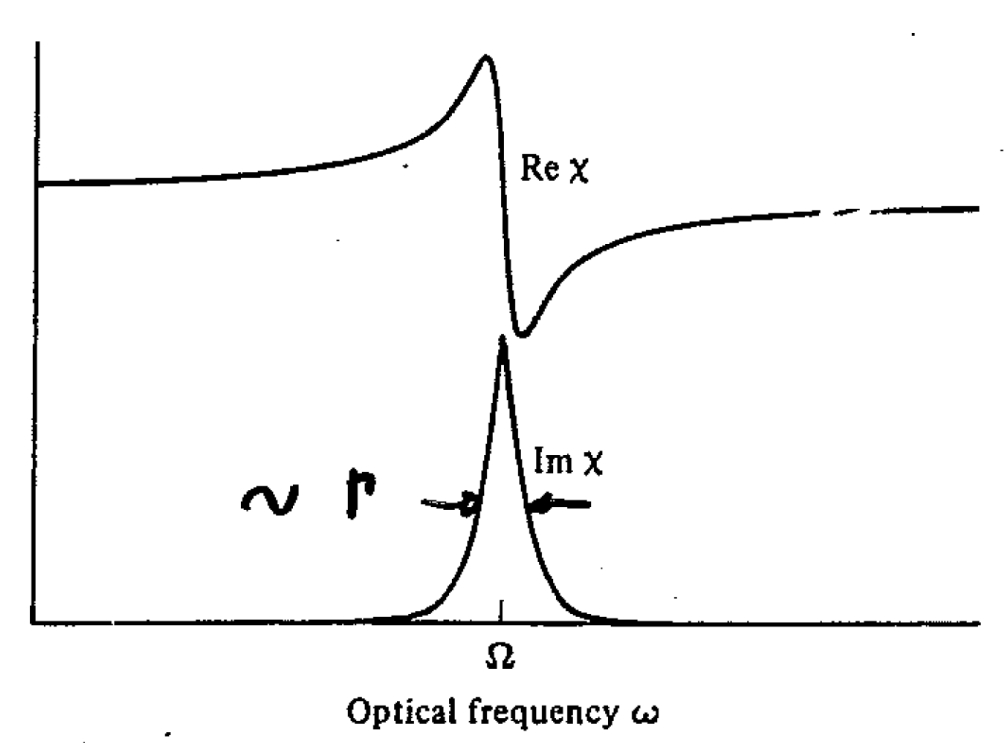
\includegraphics[width=0.8\textwidth]{image-009.png}
    \caption{Self-Phase Modulation effect showing: (top) temporal pulse shape and instantaneous power $P(T)$; (middle) nonlinear phase shift $\phi_{\text{NL}}(T)$ proportional to power; (bottom) instantaneous frequency shift $\delta\omega(T)$ showing red-shift at leading edge and blue-shift at trailing edge.}
    \label{fig:spm_effect}
\end{figure}

\subsection{SPM with Dispersion: Pulse Compression and Broadening}

When both SPM and dispersion are present, their interplay determines the pulse evolution:

\begin{itemize}[leftmargin=*]
    \item \textbf{Normal dispersion ($\beta_2 > 0$):} Higher frequencies travel slower. The blue-shifted trailing edge slows down while the red-shifted leading edge speeds up, causing additional pulse broadening.
    
    \item \textbf{Anomalous dispersion ($\beta_2 < 0$):} Higher frequencies travel faster. The blue-shifted trailing edge catches up with the red-shifted leading edge. Under certain conditions, this can lead to pulse compression or soliton formation.
\end{itemize}

\begin{physical}
\textbf{Real-world implications:}
\begin{itemize}
    \item In transmission systems, SPM-induced spectral broadening can cause adjacent channels to overlap, leading to crosstalk
    \item SPM combined with dispersion can cause severe pulse distortion, limiting transmission distance
    \item However, in the anomalous dispersion regime, SPM can be exploited to form solitons, which propagate without distortion
\end{itemize}
\end{physical}

% ==================== CROSS-PHASE MODULATION ====================
\section{Cross-Phase Modulation (XPM)}

\subsection{Physical Origin of XPM}

When two or more optical waves at different frequencies co-propagate in a fiber, each wave modulates the refractive index experienced by the other waves. This is called Cross-Phase Modulation (XPM).

\subsection{Two-Wave Interaction}

Consider two waves at frequencies $\omega_1$ and $\omega_2$ with complex envelopes $A_1(z,T)$ and $A_2(z,T)$:

\begin{equation}
    E(z,t) = \frac{1}{2}\left[A_1(z,T)e^{i(\omega_1 t - \beta_1 z)} + A_2(z,T)e^{i(\omega_2 t - \beta_2 z)} + \text{c.c.}\right]
    \label{eq:two_waves}
\end{equation}

The nonlinear polarization contains terms at both frequencies:

\begin{equation}
    P_{\text{NL}}^{(3)} = \frac{3}{8}\varepsilon_0\chi^{(3)}\left[(|A_1|^2 + 2|A_2|^2)A_1 e^{i(\omega_1 t - \beta_1 z)} + (|A_2|^2 + 2|A_1|^2)A_2 e^{i(\omega_2 t - \beta_2 z)} + \ldots\right]
    \label{eq:pnl_two_waves}
\end{equation}

\begin{physical}
\textbf{Physical Interpretation:} Each wave experiences a refractive index change due to both its own intensity (SPM term) and twice the intensity of the other wave (XPM term):

\begin{equation}
    \Delta n_1 \propto n_2 (|A_1|^2 + 2|A_2|^2)
\end{equation}
\begin{equation}
    \Delta n_2 \propto n_2 (|A_2|^2 + 2|A_1|^2)
\end{equation}

\textbf{Key observation:} The XPM effect is \textbf{twice as strong} as the SPM effect. This factor of 2 comes from the tensor structure of $\chi^{(3)}$ and is crucial for understanding nonlinear interactions in WDM systems.
\end{physical}

\subsection{Coupled NLSE for XPM}

The two waves obey coupled nonlinear Schrödinger equations:

\begin{formula}
\textbf{Coupled NLSE for XPM:}
\begin{align}
    \frac{\partial A_1}{\partial z} &= -\frac{\alpha}{2}A_1 - i\beta_{1,1}\frac{\partial A_1}{\partial T} + i\frac{\beta_{1,2}}{2}\frac{\partial^2 A_1}{\partial T^2} - i\gamma_1(|A_1|^2 + 2|A_2|^2)A_1 \label{eq:xpm_coupled1} \\
    \frac{\partial A_2}{\partial z} &= -\frac{\alpha}{2}A_2 - i\beta_{2,1}\frac{\partial A_2}{\partial T} + i\frac{\beta_{2,2}}{2}\frac{\partial^2 A_2}{\partial T^2} - i\gamma_2(|A_2|^2 + 2|A_1|^2)A_2 \label{eq:xpm_coupled2}
\end{align}

where $\beta_{k,1} = \frac{d\beta}{d\omega}\big|_{\omega_k}$ and $\beta_{k,2} = \frac{d^2\beta}{d\omega^2}\big|_{\omega_k}$ are the dispersion parameters at frequency $\omega_k$.
\end{formula}

\subsection{XPM in WDM Systems}

In Wavelength Division Multiplexing (WDM) systems, multiple channels at different wavelengths propagate simultaneously. XPM causes several impairments:

\begin{itemize}[leftmargin=*]
    \item \textbf{Spectral broadening:} Each channel's spectrum broadens due to XPM from neighboring channels
    \item \textbf{Timing jitter:} Intensity fluctuations in one channel cause phase and timing shifts in other channels
    \item \textbf{Amplitude distortion:} The combined effect of XPM and dispersion can cause amplitude fluctuations
\end{itemize}

\begin{physical}
\textbf{Real-world example:} Consider a WDM system with a strong "pump" channel and a weak "probe" channel. If we neglect the probe's SPM and assume zero dispersion for the probe:

\begin{equation}
    \frac{\partial A_{\text{probe}}}{\partial z} = -i \cdot 2\gamma |A_{\text{pump}}|^2 A_{\text{probe}}
\end{equation}

Solution:
\begin{equation}
    A_{\text{probe}}(z,T) = A_{\text{probe}}(0,T) \exp\left(-i \cdot 2\gamma \int_0^z |A_{\text{pump}}(z',T)|^2 dz'\right)
\end{equation}

This shows that the pump imposes a phase modulation on the probe that is twice as strong as if the probe were modulating itself.

\textbf{Mitigation strategies:}
\begin{itemize}
    \item Increase channel spacing to reduce XPM
    \item Use dispersion management to reduce the effective interaction length
    \item Reduce optical power (but this limits transmission distance)
\end{itemize}
\end{physical}

% ==================== FOUR-WAVE MIXING ====================
\section{Four-Wave Mixing (FWM)}

\subsection{Phase-Matched Nonlinear Interactions}

In addition to SPM and XPM, the third-order nonlinearity can generate new frequencies through Four-Wave Mixing (FWM). When two waves at frequencies $\omega_1$ and $\omega_2$ interact, they can generate waves at new frequencies:

\begin{table}[H]
    \centering
    \caption{Four-Wave Mixing frequency combinations}
    \label{tab:fwm_frequencies}
    \begin{tabular}{ccc}
        \toprule
        \textbf{Process} & \textbf{Generated Frequency} & \textbf{Propagation Constant} \\
        \midrule
        1 & $\omega_1 + \omega_1 - \omega_2 = 2\omega_1 - \omega_2$ & $2\beta_1 - \beta_2$ \\
        2 & $\omega_2 + \omega_2 - \omega_1 = 2\omega_2 - \omega_1$ & $2\beta_2 - \beta_1$ \\
        \bottomrule
    \end{tabular}
\end{table}

\begin{physical}
\textbf{Physical Interpretation:} FWM can be understood as a parametric process where two photons at one frequency are annihilated and two photons at different frequencies are created, conserving energy:

\begin{equation}
    \omega_3 + \omega_4 = \omega_1 + \omega_2
\end{equation}

However, for efficient FWM, the process must also satisfy \textbf{phase matching}:

\begin{equation}
    \beta_3 + \beta_4 = \beta_1 + \beta_2
\end{equation}

Due to chromatic dispersion, phase matching is generally not satisfied. However, at certain wavelengths (e.g., near the zero-dispersion wavelength), phase matching can occur, leading to strong FWM.

\textbf{Real-world implications in WDM systems:}
\begin{itemize}
    \item FWM generates new frequencies that can fall on existing channels, causing crosstalk
    \item FWM is strongest when channels are equally spaced and near the zero-dispersion wavelength
    \item FWM efficiency decreases rapidly with channel spacing and dispersion
\end{itemize}
\end{physical}

% ==================== SOLITONS ====================
\section{Optical Solitons}

\subsection{The Concept of Solitons}

A soliton is a special pulse shape that propagates without distortion by balancing the effects of dispersion and nonlinearity.

\begin{keypoint}
In the anomalous dispersion regime ($\beta_2 < 0$), the dispersive pulse broadening can be exactly compensated by the nonlinear pulse compression due to SPM, resulting in a pulse that maintains its shape indefinitely.
\end{keypoint}

\subsection{The Fundamental Soliton}

The fundamental (first-order) soliton is a solution to the NLSE (neglecting loss):

\begin{equation}
    \frac{\partial A}{\partial z} = i\frac{\beta_2}{2}\frac{\partial^2 A}{\partial T^2} - i\gamma |A|^2 A
    \label{eq:nlse_soliton}
\end{equation}

The fundamental soliton solution is:

\begin{formula}
\textbf{Fundamental soliton:}
\begin{equation}
    A(z,T) = A_0 \operatorname{sech}\left(\frac{T}{T_0}\right) e^{i\phi(z)}
    \label{eq:fundamental_soliton}
\end{equation}

where:
\begin{itemize}
    \item $A_0$ is the peak amplitude
    \item $T_0$ is the pulse width parameter
    \item $\operatorname{sech}(x) = \frac{2}{e^x + e^{-x}}$ is the hyperbolic secant function
    \item $\phi(z) = -\frac{1}{2}\gamma A_0^2 z$ is the accumulated phase
\end{itemize}

The soliton condition (balance between dispersion and nonlinearity) requires:
\begin{equation}
    \gamma A_0^2 |\beta_2| = \frac{1}{T_0^2}
\end{equation}

or equivalently:
\begin{equation}
    A_0^2 = \frac{1}{\gamma |\beta_2| T_0^2}
\end{equation}
\end{formula}

\begin{physical}
\textbf{Physical Interpretation:}

\textbf{How solitons work:}
\begin{enumerate}
    \item \textbf{Dispersion effect:} In anomalous dispersion ($\beta_2 < 0$), the pulse acquires a chirp such that higher frequencies (blue) are at the trailing edge and lower frequencies (red) are at the leading edge. Since blue light travels faster in anomalous dispersion, the trailing edge catches up with the leading edge, compressing the pulse.
    
    \item \textbf{SPM effect:} SPM creates the opposite chirp - red at the leading edge and blue at the trailing edge. This would normally cause the pulse to broaden in anomalous dispersion.
    
    \item \textbf{Balance:} For the fundamental soliton, these two effects exactly cancel. The pulse neither broadens nor compresses - it propagates indefinitely without changing shape.
\end{enumerate}

\textbf{Soliton parameters:}
\begin{itemize}
    \item The Full Width at Half Maximum (FWHM) is $T_{\text{FWHM}} = 1.763 \cdot T_0$
    \item The peak power must be precisely $P_0 = A_0^2 = \frac{1}{\gamma |\beta_2| T_0^2}$
    \item For a 10 ps soliton in standard fiber ($\beta_2 \approx -20$ ps$^2$/km, $\gamma \approx 1.3$ W$^{-1}$km$^{-1}$): $P_0 \approx 3.8$ mW
\end{itemize}

\textbf{Real-world significance:} Soliton transmission was proposed in the 1980s as a way to overcome dispersion limitations in long-haul fiber optic systems. While modern systems use other techniques (dispersion compensation, coherent detection), solitons remain important in ultrafast optics and supercontinuum generation.
\end{physical}

\subsection{Higher-Order Solitons}

When the peak power is increased by a factor of $N^2$ (where $N$ is an integer), higher-order solitons form:

\begin{equation}
    A_0^2 = \frac{N^2}{\gamma |\beta_2| T_0^2}
\end{equation}

\begin{physical}
\textbf{Physical Behavior:} Higher-order solitons ($N > 1$) exhibit periodic evolution. The pulse shape oscillates between compression and broadening with a period called the \textbf{soliton period}:

\begin{equation}
    z_0 = \frac{\pi T_0^2}{2|\beta_2|}
\end{equation}

At $z = z_0/2$, the pulse is maximally compressed. At $z = z_0$, the pulse returns to its original shape. This periodic behavior continues indefinitely (in the absence of loss and higher-order effects).
\end{physical}

\subsection{Soliton Perturbations and Stability}

In real fibers, solitons are subject to perturbations:

\begin{itemize}[leftmargin=*]
    \item \textbf{Fiber loss:} Causes soliton amplitude to decay, requiring periodic amplification
    \item \textbf{Third-order dispersion ($\beta_3$):} Causes soliton to shed energy as dispersive waves
    \item \textbf{Raman effect:} Causes soliton to shift to longer wavelengths (soliton self-frequency shift)
    \item \textbf{Amplifier noise:} Can cause timing jitter and amplitude fluctuations
\end{itemize}

\begin{physical}
\textbf{Practical soliton systems:} Despite these perturbations, solitons are remarkably robust. They can recover from small perturbations and continue propagating. This stability makes them attractive for long-distance transmission, though modern systems typically use other approaches due to complexity and cost considerations.
\end{physical}

% ==================== MODULATION INSTABILITY ====================
\section{Modulation Instability (MI)}

\subsection{Physical Origin of MI}

Modulation Instability is a phenomenon where a continuous wave (CW) or quasi-CW signal becomes unstable to small perturbations in the anomalous dispersion regime. Small amplitude or phase modulations grow exponentially, breaking up the CW into a train of pulses.

\begin{keypoint}
MI is the temporal analog of spatial self-focusing. It arises from the interplay between SPM and anomalous dispersion, and is closely related to soliton formation.
\end{keypoint}

\subsection{Linear Stability Analysis}

Consider a CW with a small perturbation:

\begin{equation}
    A(z,T) = \sqrt{P_0}(1 + a(z,T))e^{-i\gamma P_0 z}
    \label{eq:mi_ansatz}
\end{equation}

where $P_0$ is the CW power and $|a| \ll 1$ is a small perturbation.

Substituting into the NLSE and linearizing in $a$:

\begin{equation}
    \frac{\partial a}{\partial z} = i\frac{\beta_2}{2}\frac{\partial^2 a}{\partial T^2} - i\gamma P_0(a + a^*)
    \label{eq:mi_linearized}
\end{equation}

Assume a perturbation of the form:

\begin{equation}
    a(z,T) = a_1 e^{i(\Omega T - Kz)} + a_2^* e^{-i(\Omega T - K^*z)}
    \label{eq:mi_perturbation}
\end{equation}

where $\Omega$ is the modulation frequency and $K$ is the growth rate.

\subsection{Dispersion Relation and Gain Spectrum}

Solving the linearized equation yields the dispersion relation:

\begin{formula}
\textbf{MI dispersion relation:}
\begin{equation}
    K = \pm\sqrt{-\frac{\beta_2^2\Omega^4}{4} + \gamma P_0 \beta_2 \Omega^2}
    \label{eq:mi_dispersion}
\end{equation}

For MI to occur, $K$ must have an imaginary part (exponential growth). This requires:

\begin{equation}
    -\frac{\beta_2^2\Omega^4}{4} + \gamma P_0 \beta_2 \Omega^2 > 0
\end{equation}

which simplifies to:
\begin{equation}
    \beta_2 < 0 \quad \text{and} \quad \Omega^2 < \frac{4\gamma P_0}{|\beta_2|}
    \label{eq:mi_condition}
\end{equation}
\end{formula}

\begin{physical}
\textbf{Physical Interpretation:}

\textbf{MI condition:} MI only occurs in the \textbf{anomalous dispersion regime} ($\beta_2 < 0$). In normal dispersion ($\beta_2 > 0$), the CW is stable.

\textbf{Gain spectrum:} The MI gain $g(\Omega) = 2\operatorname{Im}(K)$ is:

\begin{equation}
    g(\Omega) = 2\sqrt{\gamma P_0 |\beta_2| \Omega^2 - \frac{\beta_2^2 \Omega^4}{4}}
\end{equation}

This gain is maximum at:
\begin{equation}
    \Omega_{\max} = \sqrt{\frac{2\gamma P_0}{|\beta_2|}}
\end{equation}

with maximum gain:
\begin{equation}
    g_{\max} = 2\gamma P_0
\end{equation}
\end{physical}

\begin{figure}[H]
    \centering
    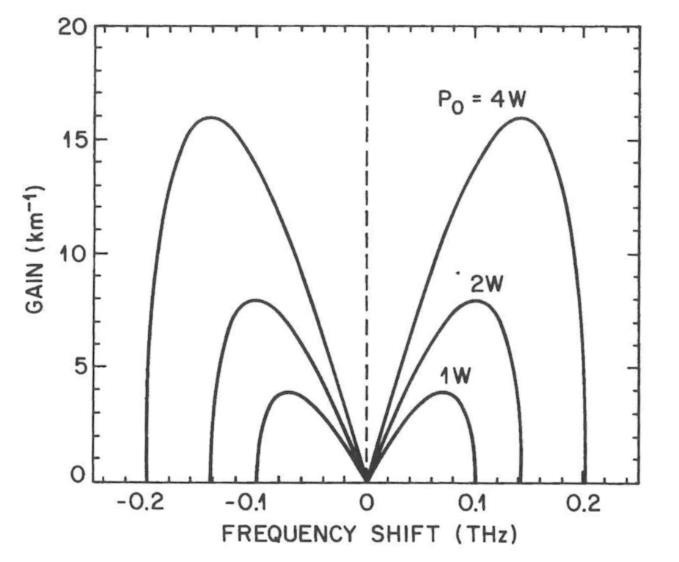
\includegraphics[width=0.7\textwidth]{image-014.png}
    \caption{Modulation Instability gain spectrum $g(\Omega)$ as a function of modulation frequency $\Omega$. The gain is maximum at $\Omega_{\max}$ and drops to zero at the cutoff frequency $\Omega_c = 2\sqrt{\gamma P_0/|\beta_2|}$. Only perturbations within the gain bandwidth experience exponential growth.}
    \label{fig:mi_gain}
\end{figure}

\begin{physical}
\textbf{Physical mechanism of MI:}

\begin{enumerate}
    \item A small intensity modulation creates regions of higher and lower power
    \item Through SPM, the high-power regions experience larger phase shifts
    \item This creates a phase modulation that converts to amplitude modulation through dispersion
    \item In anomalous dispersion, this feedback is positive, causing the modulation to grow exponentially
    \item Eventually, the CW breaks up into a periodic train of pulses
\end{enumerate}

\textbf{Real-world applications and implications:}

\textbf{Negative effects:}
\begin{itemize}
    \item In transmission systems, MI can cause CW or quasi-CW signals to break up, degrading signal quality
    \item MI can seed other nonlinear processes like FWM
\end{itemize}

\textbf{Positive applications:}
\begin{itemize}
    \item MI can be used to generate ultrashort pulse trains from CW lasers
    \item MI is exploited in supercontinuum generation
    \item MI-based parametric amplifiers can provide wavelength conversion and signal amplification
\end{itemize}

\textbf{Example:} For a CW with power $P_0 = 100$ mW in standard fiber ($\beta_2 = -20$ ps$^2$/km, $\gamma = 1.3$ W$^{-1}$km$^{-1}$):
\begin{itemize}
    \item Maximum gain frequency: $\Omega_{\max} = 2\pi \times 2.56$ THz
    \item Maximum gain: $g_{\max} = 260$ km$^{-1}$ (very strong!)
    \item After 1 km, a small perturbation at $\Omega_{\max}$ grows by a factor of $e^{g_{\max} \cdot 1 \text{ km}/2} \approx 10^{56}$ (in practice, nonlinear saturation limits this growth)
\end{itemize}
\end{physical}

\subsection{MI Sidebands and Pulse Formation}

As MI develops, sidebands appear in the optical spectrum at frequencies $\omega_0 \pm \Omega_{\max}$. In the time domain, this corresponds to a periodic intensity modulation that eventually evolves into a train of soliton-like pulses.

\begin{figure}[H]
    \centering
    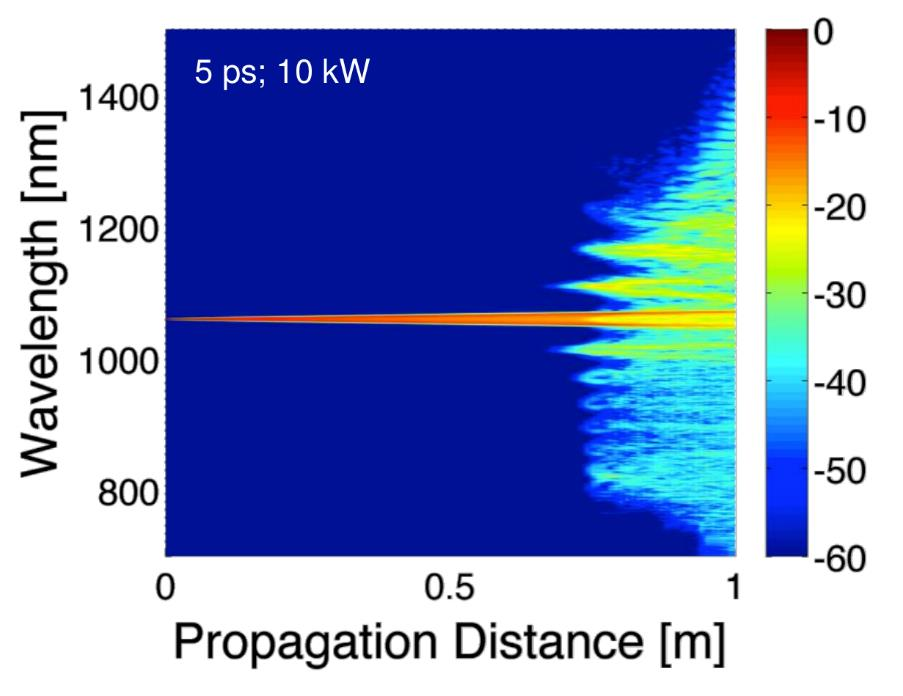
\includegraphics[width=0.8\textwidth]{image-015.png}
    \caption{Evolution of Modulation Instability: (a) Initial CW with small noise; (b) Growth of MI sidebands in the spectrum; (c) Formation of periodic pulse train in time domain; (d) Further evolution showing pulse compression and soliton formation.}
    \label{fig:mi_evolution}
\end{figure}

% ==================== POLARIZATION EFFECTS ====================
\section{Polarization Effects in Nonlinear Propagation}

\subsection{Polarization-Dependent Nonlinearity}

In anisotropic fibers (such as polarization-maintaining fibers), the polarization state of light affects the nonlinear response. For two orthogonal polarization components $A_x$ and $A_y$:

\begin{formula}
\textbf{Coupled NLSE with polarization effects:}
\begin{align}
    \frac{\partial A_x}{\partial z} &= -\frac{\alpha}{2}A_x - i\beta_{x,1}\frac{\partial A_x}{\partial T} + i\frac{\beta_{x,2}}{2}\frac{\partial^2 A_x}{\partial T^2} - i\gamma\left(|A_x|^2 + \frac{2}{3}|A_y|^2\right)A_x - i\frac{\gamma}{3}A_x^* A_y^2 e^{-i\Delta\beta z} \label{eq:pol_nlse_x} \\
    \frac{\partial A_y}{\partial z} &= -\frac{\alpha}{2}A_y - i\beta_{y,1}\frac{\partial A_y}{\partial T} + i\frac{\beta_{y,2}}{2}\frac{\partial^2 A_y}{\partial T^2} - i\gamma\left(|A_y|^2 + \frac{2}{3}|A_x|^2\right)A_y - i\frac{\gamma}{3}A_y^* A_x^2 e^{i\Delta\beta z} \label{eq:pol_nlse_y}
\end{align}

where $\Delta\beta = \beta_x - \beta_y$ is the birefringence.
\end{formula}

\begin{physical}
\textbf{Physical Interpretation:}

\textbf{SPM and XPM terms:} Each polarization component experiences:
\begin{itemize}
    \item SPM from its own intensity: $|A_x|^2$ or $|A_y|^2$
    \item XPM from the orthogonal polarization: $\frac{2}{3}|A_y|^2$ or $\frac{2}{3}|A_x|^2$
\end{itemize}

Note that the XPM coefficient is $\frac{2}{3}$ instead of 2 (as in the case of different frequencies). This factor comes from the tensor structure of $\chi^{(3)}$ for orthogonal polarizations.

\textbf{Four-Wave Mixing terms:} The terms $A_x^* A_y^2 e^{-i\Delta\beta z}$ and $A_y^* A_x^2 e^{i\Delta\beta z}$ represent FWM between the two polarizations. These terms are phase-mismatched by the birefringence $\Delta\beta$ and are usually negligible in highly birefringent fibers.

\textbf{Real-world implications:}
\begin{itemize}
    \item In standard single-mode fibers with low birefringence, polarization effects can cause additional signal distortion
    \item Polarization mode dispersion (PMD) combined with nonlinearity can lead to complex pulse distortion
    \item In polarization-maintaining fibers, the large birefringence suppresses FWM between polarizations
\end{itemize}
\end{physical}

% ==================== SUMMARY ====================
\section{Summary and Conclusions}

\subsection{Key Concepts}

This document has covered the fundamental aspects of nonlinearity in optical fibers:

\begin{enumerate}[leftmargin=*]
    \item \textbf{Origin of nonlinearity:} The mechanical oscillator model shows how the anharmonic restoring force leads to nonlinear polarization $P = \varepsilon_0(\chi^{(1)}E + \chi^{(3)}E^3 + \ldots)$
    
    \item \textbf{Kerr effect:} The intensity-dependent refractive index $n = n_0 + n_2 I$ is the foundation of all nonlinear effects in silica fibers
    
    \item \textbf{NLSE derivation:} The Nonlinear Schrödinger Equation captures the interplay between dispersion, loss, and nonlinearity:
    \begin{equation*}
        \frac{\partial A}{\partial z} = -\frac{\alpha}{2}A + i\frac{\beta_2}{2}\frac{\partial^2 A}{\partial T^2} - i\gamma |A|^2 A
    \end{equation*}
    
    \item \textbf{Self-Phase Modulation (SPM):} Causes frequency chirp and spectral broadening without changing pulse shape
    
    \item \textbf{Cross-Phase Modulation (XPM):} In WDM systems, channels modulate each other with twice the strength of SPM
    
    \item \textbf{Solitons:} In anomalous dispersion, the balance between dispersion and nonlinearity enables distortion-free propagation
    
    \item \textbf{Modulation Instability (MI):} CW signals break up into pulse trains in anomalous dispersion regime
\end{enumerate}

\subsection{Practical Design Considerations}

\begin{table}[H]
    \centering
    \caption{Summary of nonlinear effects and their impact}
    \label{tab:nonlinear_summary}
    \begin{tabularx}{\textwidth}{lXX}
        \toprule
        \textbf{Effect} & \textbf{Key Parameters} & \textbf{Mitigation/Exploitation} \\
        \midrule
        SPM & $\gamma$, $P_0$, $L_{\text{eff}}$ & Reduce power, increase $A_{\text{eff}}$, or exploit for solitons \\
        \addlinespace
        XPM & $\gamma$, channel spacing, dispersion & Increase channel spacing, dispersion management \\
        \addlinespace
        FWM & $\gamma$, $P_0$, $\beta_2$, channel spacing & Operate away from zero-dispersion, unequal channel spacing \\
        \addlinespace
        MI & $\gamma$, $P_0$, $\beta_2$ & Avoid anomalous dispersion for CW, or exploit for pulse generation \\
        \bottomrule
    \end{tabularx}
\end{table}

\subsection{Future Directions}

Nonlinear fiber optics continues to be an active research area with applications in:

\begin{itemize}[leftmargin=*]
    \item Ultrafast pulse generation and shaping
    \item Supercontinuum sources for spectroscopy and imaging
    \item All-optical signal processing
    \item Quantum optics and photon pair generation
    \item High-power fiber lasers
\end{itemize}

Understanding the mathematical foundations and physical mechanisms of nonlinear effects is essential for both designing robust transmission systems and developing novel photonic devices.

\end{document}
